Il menu di un sito web è fondamentale nell'esperienza di navigazione: se l'utente incontrasse difficoltà nel suo utilizzo, potrebbe decidere di abbandonare la pagina sulla quale si trova.

\paragraph*{Primo impatto} Non benissimo. La struttura di primo livello del menu lascia abbastanza perplessi: mentre le voci \textit{Sistemi e Prodotti} e \textit{Contatti} sono chiare e intuitive, lo stesso non si può dire di \textit{Spazi che parlano di te} e \textit{Spazi che parlano di noi}. Queste ultime riprendono chiaramente il motto dell'azienda, ma non risulta per niente chiaro a cosa indirizzino: l'utente è quindi costretto a fare \textit{click gambling}, nella speranza di trovare ulteriori indizi. Il menu è fondamentale per favorire un'esperienza di navigazione positiva per l'utente: metterci slogan non è sicuramente la migliore delle scelte.\\
Una volta che ci si sposta col mouse sopra il menu, compare una freccia verso il basso che suggerisce la presenza di un secondo livello. Bene che ciò sia indicato.\\
Apprezzabile l'idea di spiegare ulteriormente il significato di ogni voce, ma ci sono degli svantaggi:
\begin{itemize}	
	\item Il menu occupa in larghezza tutto lo schermo. Se le voci fossero più chiare, si potrebbe risparmiare spazio togliendo l'ulteriore spiegazione. Si potrebbe quindi far aprire e chiudere il menu senza necessitare di un singolo click da parte dell'utente.
	\item Si presenta spesso la scritta \textit{"Entra nella pagina X"} quando i selettori del menu sono già cliccabili e conducono alla stessa pagina (\autoref{fig:menu_2lvl}).
\end{itemize}

\begin{figure}
	\centering
	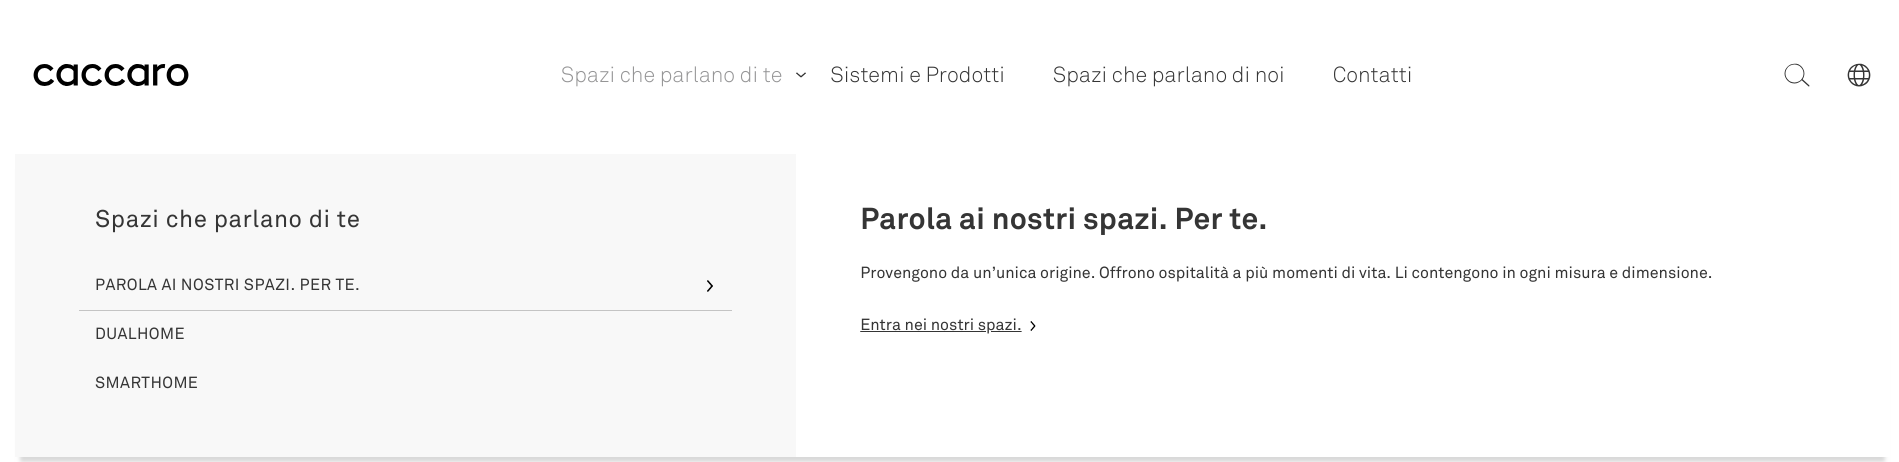
\includegraphics[width=\textwidth]{sez/Elementi_Comuni/img/menu_STD.png}
	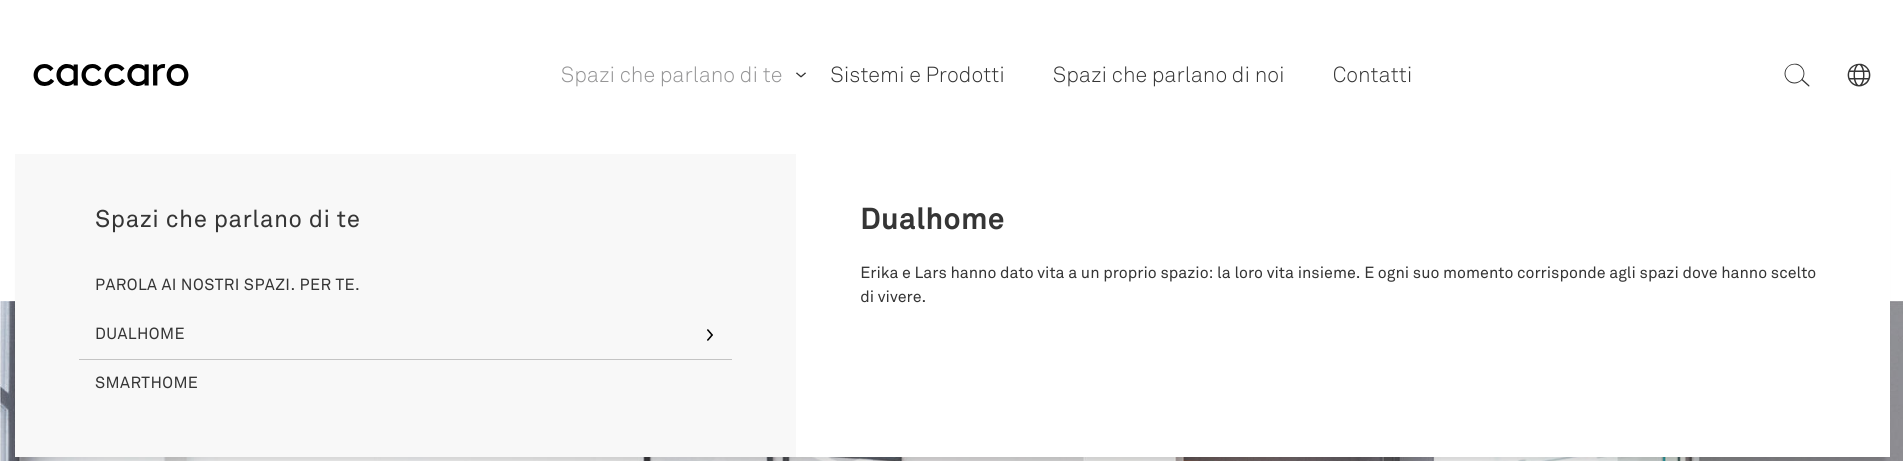
\includegraphics[width=\textwidth]{sez/Elementi_Comuni/img/menu_STD2.png}
	\caption{Menu a due livelli: perché nel primo c'è un ulteriore link e nel secondo no?}
	\label{fig:menu_2lvl}
\end{figure}

\paragraph*{Struttura} A seconda della voce di menu selezionata, ci possiamo trovare davanti ad un menu con uno, due o tre livelli (nel conto è incluso anche il livello immediatamente visibile). Considerano che un numero di livelli superiore a due può far innervosire l'utente, sarebbe il caso di modificare i menu con tre livelli (\autoref{fig:menu_3lvl}).

\begin{figure}
	\centering
	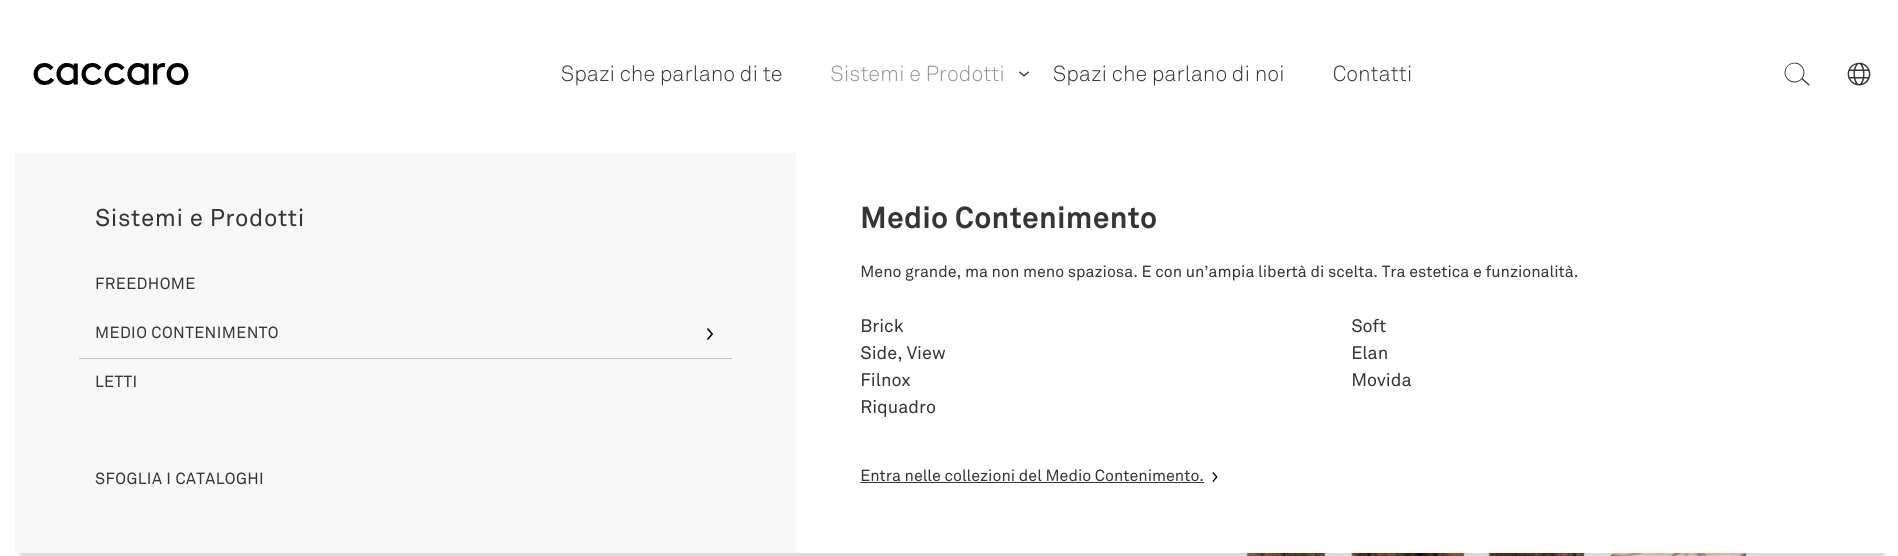
\includegraphics[width=\textwidth]{sez/Elementi_Comuni/img/menu_3lvl.png}
	\caption{Esempio di menu a tre livelli}
	\label{fig:menu_3lvl}
\end{figure}

\paragraph*{Fault-Tolerance} Il menù è tendenzialmente \textit{fault-tolerant}. L'espansione e la compressione di una voce di primo livello richiedono un click sulla voce stessa: questo evita una possibile chiusura accidentale, ma ha lo svantaggio (non banale) di richiedere un click in più da parte dell'utente. 
Le voci di secondo livello, invece, aprono il pannello sulla destra. Anche spostando il mouse fuori dalla voce il pannello resta aperto, molto bene.

\paragraph*{Icone} Sono presenti in alto a destra due icone:
\begin{itemize}
\item \textbf{Lente di ingrandimento:} \`E la classica icona per la ricerca, molto familiare all'utente. Bene.
\item \textbf{Globo stilizzato:} \`E l'icona per cambiare lingua al sito, sono disponibili Italiano e Inglese. Non è forse familiare all'utente come lo è la lente di ingrandimento, però è sicuramente un buon compromesso. Si sarebbe potuto accompagnarla con una scritta IT/EN, o ancora meglio, mostrare la lingua corretta in base all'indirizzo IP, ma sono solo dettagli.
\end{itemize}